%%%%%%%%%%%%%%%%%%%%%%%%%%%%%%%%%%%%%%%%%
% University Assignment Title Page 
% LaTeX Template
% Version 1.0 (27/12/12)
%
% This template has been downloaded from:
% http://www.LaTeXTemplates.com
%
% Original author:
% WikiBooks (http://en.wikibooks.org/wiki/LaTeX/Title_Creation)
%
% License:
% CC BY-NC-SA 3.0 (http://creativecommons.org/licenses/by-nc-sa/3.0/)
% 
% Instructions for using this template:
% This title page is capable of being compiled as is. This is not useful for 
% including it in another document. To do this, you have two options: 
%
% 1) Copy/paste everything between \begin{document} and \end{document} 
% starting at \begin{titlepage} and paste this into another LaTeX file where you 
% want your title page.
% OR
% 2) Remove everything outside the \begin{titlepage} and \end{titlepage} and 
% move this file to the same directory as the LaTeX file you wish to add it to. 
% Then add %%%%%%%%%%%%%%%%%%%%%%%%%%%%%%%%%%%%%%%%%
% University Assignment Title Page 
% LaTeX Template
% Version 1.0 (27/12/12)
%
% This template has been downloaded from:
% http://www.LaTeXTemplates.com
%
% Original author:
% WikiBooks (http://en.wikibooks.org/wiki/LaTeX/Title_Creation)
%
% License:
% CC BY-NC-SA 3.0 (http://creativecommons.org/licenses/by-nc-sa/3.0/)
% 
% Instructions for using this template:
% This title page is capable of being compiled as is. This is not useful for 
% including it in another document. To do this, you have two options: 
%
% 1) Copy/paste everything between \begin{document} and \end{document} 
% starting at \begin{titlepage} and paste this into another LaTeX file where you 
% want your title page.
% OR
% 2) Remove everything outside the \begin{titlepage} and \end{titlepage} and 
% move this file to the same directory as the LaTeX file you wish to add it to. 
% Then add %%%%%%%%%%%%%%%%%%%%%%%%%%%%%%%%%%%%%%%%%
% University Assignment Title Page 
% LaTeX Template
% Version 1.0 (27/12/12)
%
% This template has been downloaded from:
% http://www.LaTeXTemplates.com
%
% Original author:
% WikiBooks (http://en.wikibooks.org/wiki/LaTeX/Title_Creation)
%
% License:
% CC BY-NC-SA 3.0 (http://creativecommons.org/licenses/by-nc-sa/3.0/)
% 
% Instructions for using this template:
% This title page is capable of being compiled as is. This is not useful for 
% including it in another document. To do this, you have two options: 
%
% 1) Copy/paste everything between \begin{document} and \end{document} 
% starting at \begin{titlepage} and paste this into another LaTeX file where you 
% want your title page.
% OR
% 2) Remove everything outside the \begin{titlepage} and \end{titlepage} and 
% move this file to the same directory as the LaTeX file you wish to add it to. 
% Then add %%%%%%%%%%%%%%%%%%%%%%%%%%%%%%%%%%%%%%%%%
% University Assignment Title Page 
% LaTeX Template
% Version 1.0 (27/12/12)
%
% This template has been downloaded from:
% http://www.LaTeXTemplates.com
%
% Original author:
% WikiBooks (http://en.wikibooks.org/wiki/LaTeX/Title_Creation)
%
% License:
% CC BY-NC-SA 3.0 (http://creativecommons.org/licenses/by-nc-sa/3.0/)
% 
% Instructions for using this template:
% This title page is capable of being compiled as is. This is not useful for 
% including it in another document. To do this, you have two options: 
%
% 1) Copy/paste everything between \begin{document} and \end{document} 
% starting at \begin{titlepage} and paste this into another LaTeX file where you 
% want your title page.
% OR
% 2) Remove everything outside the \begin{titlepage} and \end{titlepage} and 
% move this file to the same directory as the LaTeX file you wish to add it to. 
% Then add \input{./title_page_1.tex} to your LaTeX file where you want your
% title page.
%
%%%%%%%%%%%%%%%%%%%%%%%%%%%%%%%%%%%%%%%%%
%\title{Title page with logo}
%----------------------------------------------------------------------------------------
%	PACKAGES AND OTHER DOCUMENT CONFIGURATIONS
%----------------------------------------------------------------------------------------

\documentclass[12pt]{article}
\usepackage[english]{babel}
\usepackage[utf8x]{inputenc}
\usepackage{amsmath}
\usepackage{graphicx}
\usepackage[colorinlistoftodos]{todonotes}
\usepackage{setspace}
\usepackage{algpseudocode}
\usepackage{algorithm}
\usepackage{amsthm} \usepackage{color, colortbl}
\usepackage{cite}
\begin{document}

\begin{titlepage}

\newcommand{\HRule}{\rule{\linewidth}{0.5mm}} % Defines a new command for the horizontal lines, change thickness here

\center % Center everything on the page
 
%----------------------------------------------------------------------------------------
%	HEADING SECTIONS
%----------------------------------------------------------------------------------------

\textsc{\LARGE EECS 227C}\\[1.0cm] % Name of your university/college
\textsc{\Large Course Project}\\[2.0cm] % Major heading such as course name

%----------------------------------------------------------------------------------------
%	TITLE SECTION
%----------------------------------------------------------------------------------------

% \HRule \\[0.3cm]
\singlespacing \huge \textbf{Mirror Descent Method for Online Portfolio Allocation with Hedging}
\\[0.2cm] % Title of your document
\HRule \\[2.0cm]
 
%----------------------------------------------------------------------------------------
%	AUTHOR SECTION
%----------------------------------------------------------------------------------------

\begin{minipage}{0.4\textwidth}
\begin{flushleft} \large
\emph{Name:}\\
Ying \textsc{Cao}\\
Shiman \textsc{Ding}\\
Renyuan \textsc{Xu}
\end{flushleft}
\end{minipage}
~
\begin{minipage}{0.4\textwidth}
\begin{flushright} \large
\emph{SID:} \\
25937400\\
24104985\\
25945145
\end{flushright}
\end{minipage}\\[2.5cm]

% If you don't want a supervisor, uncomment the two lines below and remove the section above
%\Large \emph{Author:}\\
%John \textsc{Smith}\\[3cm] % Your name

%----------------------------------------------------------------------------------------
%	DATE SECTION
%----------------------------------------------------------------------------------------

{\large \today}\\[2cm] % Date, change the \today to a set date if you want to be precise

%----------------------------------------------------------------------------------------
%	LOGO SECTION
%----------------------------------------------------------------------------------------

% \includegraphics{logo.png}\\[1cm] % Include a department/university logo - this will require the graphicx package
 
%----------------------------------------------------------------------------------------

\vfill % Fill the rest of the page with whitespace

\end{titlepage}

\onehalfspacing
\begin{abstract}
Online portfolio selection is a fundamental problem in computational finance, which has been extensively studied across several research communities, including finance, statistics, artificial intelligence, machine learning, and data mining, etc.
In this project we incorporate structured hedging, price mean reversion, and other loss penalty terms into the model of portfolio management. We present a formulation for hedging online resource allocations with leverage and propose mirror descent method to solve the problem sequentially. We implement our model on SP500 and DJIA dataset, and compare our algorithm with a recently proposed algorithm, SHREAL, by \cite{johnson2015structured} to see the difference.
\end{abstract}


\section{Introduction}

Online resource allocation is a fundamental problem problem in mathematical finance. It is complicated since the optimal portfolio selection
strategy should take into consideration not only maximizing the expected return, but also the risk management of the portfolio. And it becomes a more challenging problem when we allow for leveraging and transaction costs.\\

\noindent Previous research \cite{johnson2015online,blum1999universal,kalai2003efficient} has been focusing extensively on portfolio management under limited budget. That is, they only consider strategies with resources on hand. But in reality, especially in stock market, people can borrow additional money at certain risk to apply leverage and increase return. Such leverage provides us more flexibility in management, as well as more risk since profits and losses are all magnified. One common method to control risk is to hedge. Specifically for stock markets, stocks are more often correlated than independent. Taking advantage of these correlations, we can invest in the same or opposite directions in different stocks to hedge risk. For example, HSBA-LN and HSBC are two stocks based on the same underlying company, hence their returns are highly correlated. Then if we long position in one and short position in the other, the risk is almost perfectly hedged, which protects our investment if market crashes.\\

\noindent In this paper, we incorporate different regularization terms into portfolio management, including a correlation graph of hedging, price mean reversion and momentum regularization, loss function for profits and losses. We also analyze our algorithm under different transaction costs on different datasets.

\section{Precursors}
\subsection{Long and Short Positions}
For each stock, we can hold two positions: long and short. A \textbf{long position} means we buy the stock with our money on hand, and if the stock price goes up, we make some profit. In contrast, a \textbf{short position} is taken when we borrowed some stock and sell on the market. And one will profit if its price decreases. In this paper, we assume both long and short positions can be taken at any number of shares.

\subsection{Hedging and Leverage}
As we mentioned before, \textbf{hedging} takes advantage of the structural dependencies between the assets and offsets the risk of a particular allocation by utilizing both short and long positions. It is specially important when market crashes. Given any $n$ stocks, We build a correlation graph of $2n$ nodes and $2n\cdot n$ edges, where each stock is associated with two nodes, one for long position and one for short position. The graph is bipartite with natural partition of long and short positions. An edge is made between any two nodes with opposite positions and the weight of the edge is the correlation of the two stocks of the nodes (could be the same). If two stocks are highly positive correlated, we want our portfolio to take opposite directions in them so as to lower risk in the portfolio.\\ 

\noindent \textbf{Leverage} is another useful tool in financial  market, where we borrow money from some external resource, say bank, to increase allocation power. It helps to amply the potential return at the cost of exposure to higher risk in our investment. A common practice in stock market is to buy on margins. This is to buy stocks using cash borrowed, and is usually operated by putting some money into a margin account. Interest is also charged on the loan.

\subsection{Mean Reversion}
Price change of a stock reflects market's view on its fair value. Price goes up if the current price is under people's expectation and vice versa. But in many scenarios, market tends to overreact to news or other event occurring in the market. That is also intuitive to what we observe in daily life, when the price of a stock goes up dramatically, it is more like to decrease next day, which is called \textbf{mean reversion} phenomenon of stock price. Extensive studies, such as \cite{li2012line}, have shown that mean reversion strategies may better fit the market and give better empirical results. This inspires us to includes a regulation term to  capture this property in our formulation.

\subsection{Price Momentum }
\textbf{Price momentum} is the opposite action of mean reversion property. The idea behind this theory is simple that investors will buy past winners and sell past losers so that price is more likely to keep moving in the same direction than to change directions. This theory helps lower noises and smooth our management of portfolio. It is specially useful when traders want to execute huge volume while minimize price impact on the market. 


\section{Problem Formulation}
In this section, we introduce a framework adopted from [1] for structured hedging with leverage, and consider the online resource allocation problem under such structured hedging.

\subsection{Some Notations}
    \noindent For any $n$ stocks, our goal is to find an allocation $p \in P \subset R^{2n}$ which determines how to split up a resource among long and short positions over the $n$ stocks such that a certain loss function $f(p)$ is minimized. Denote the set of of index $l=\{1,...,n\}$ and $s=\{n+1, n+2, ... 2n\}$ as the long and short positions in $p$ and let $D_l$ and $D_s$ be $2n$ by $2n$ diagonal matrix with $D_l(i,i)=1, \forall i\in l$, $D_s(i,i)=1, \forall i\in s$. Let $q_l = D_lp \geq 0, q_s = D_sp \leq
    0$, in which $q_l \geq 0$ and $q_s \leq 0$ is the long only and short only vectors. The basic idea for hedging is place money in opposing positions and different assets. We can make use of the structural dependencies between stocks to effectively control risk by constructing a correlation Matrix $W$ as discussed above.\\

    \noindent We consider a stock market consisting of $n$ stocks $\{s_1,...s_n\}$ over $T$ periods. In our numerical experiments, we consider a period to be a day, but same analysis holds for any other valid period definition. Let $x_t(i)$ denote the \textbf{price relative} of stock $s_i$ in day $t$, which is the ratio of current price over previous price. Clearly, $x_t(i) > 1$ means an increase in price, and $x_t(i) < 1$ means a decrease in price. Let 
    $\hat{x_t} = [x_t(1),...x_t(n)]^T$ denote the vector of price relatives for day $t$. For the convenience of formulation, we denote $x_t = [\hat{x_t}, \hat{x_t}]^T$. The portfolio on day $t$ is $p_t = [p_t(1),...p_t(2n)]^T$, in which the first $l$ positions are for long-only allocation, and the last $s$ positions are for short-only allocation.\\

    \noindent Assume bank interest is $r$ per day. At the end of the day $t$, the multiplicative gain in wealth is :
    $$\phi (t) = q_l^Tx_t + (1-q_l^T\textbf{1})(1+r) + q_s^T(x_t-1+r)$$
    in which the first item is the gain from long position, the second item is the gain or loss from saving or leverage, and the third item is the gain from short positions. We assume the change in price are bounded as $ 0 < 1 - B_l < x_t < 1 + B_s < \infty$ to guarantee the positiveness of this multiplicative gain. Therefore, we can put constrains $q_l \geq 0, q_s \leq 0, a^Tp \leq \frac{1+r}{r+B_l}$ on $p$ to ensure we are not going to have negative wealth at the end of a day after selling out all stocks and paying back money borrowed from bank. In the constraints, according to \cite{johnson2015structured}, for vector $a$, we set the first $l$ elements are equal to 1 and the last $s$ elements are equal to $-\frac{B_s+r}{B_l+r}$.\\ 


\subsection{Loss functions}

    \noindent In order to formulate the portfolio management problem as an online convex optimization. We first need to define a loss function for day $t$. Our loss function consists four parts:
    $$l_t(p) = \xi l_t^{0}(p) + \lambda l_t^{d}(p) + \alpha l_t^{r}(p) + \beta l_t^{m}(p)$$

    \begin{itemize}

        \item The first term $l_t^0(p)$ is the negative logrithm of the multiplicative gain of day $t$.
            $$l_t^{0}(p) = -log(a_1q_l^Tx_t + a_2q_s^T(x_t-1+r) + (1-q_l^T\textbf{1})(1+r))$$
            in which $a_1, a_2$ are the weights put on long positions and short positions respectively to control their importance.\\

        \item The second term $l_t^d(p)$ is the hedging penalty function based on estimated structural dependencies.
            $$l_t^{d}(p) = \sum_{i=1}^n\sum_{j=1+n, j\neq i+n}^{2n} Corr(i,j)(q_l(i)+q_s(j))^2$$
            in which $Corr(i,j)$ is the estimated correlation between stock $i$ and $j$ based on historical data from the previous $\delta$ days. When $Corr(i,j)$ is large, we minimize this loss by making the opposing positions of $i,j$ close. This minimization can effectively encourage hedging. This loss term can be rewritten in the following matrix form:
            $$l_t^{d}(p) = p^TLp$$
            in which $L=U+D$, $U = [0, W; W, 0]$. $W$ is the estimated correlation matrix, $D$ is a diagonal matrix with $D(i,i)=\sum_j U(i,j)$.

        \item The third term $l_t^r(p)$ is the mean reversion penalty based on the the mean reversion theory.
            $$l_t^r(p)=(x_{t} - 1)^Tp$$

        \item Finally, the fourth term $l_t^m(p_t)$ is the momentum penalty:
            $$l_t^m(p)=\frac{1}{2}||p-2p_{t}+p_{t-1})||^2$$

    \end{itemize}


    \noindent Clearly, this loss function is convex, take the derivative of $l_t(p)$, we have:
\begin{align}\nonumber
\nabla l_t(p) & = \xi \frac{\alpha_1D_l^Tx_t+\alpha_2D_s^T(x_t-1+r)-D_l^T\textbf{1}(1+r)}{\alpha_1p^TD_l^Tx_t+\alpha_2p^TD_s^T(x_t-1+r)+(1-p^TD_l^T\textbf{1})(1+r)} \\ &\  \ + \lambda (L^T+L)p + \alpha (x_{t}-1) + \beta (p - 2p_{t} + p_{t-1})
\end{align}

\subsection{Regularized linear game}

    By a first-order Taylor expansion of the defined lodd function $\_t$ at $p_t$, we formulate the portfolio selection problem as follows:

    \begin{align} \label{1}
    p_{t+1} = argmin_{q_l \geq 0, q_s \leq 0, a^Tp\leq \frac{1+r}{B_l+r}} \bigg\{\eta_t \nabla l_t(p_t)^Tp + \frac{1}{2}||p-p_t||_2^2\bigg\} 
    \end{align}
    \noindent Since $l_t(p)$ is strongly convex, we can use mirror descent with a step size of $O(\frac{1}{t})$ to ensure a regret bound of $O(log T)$. That is,

    $$\hat{L}_n - L_n^{\star} \leq O(log T)$$

\section{Mirror Descent Algorithm}

    \begin{algorithm}
        \caption{Proposed Algorithm for Structural Hedging}
        \begin{algorithmic}
            \State $\xi, \alpha_1, \alpha_2, \lambda, \alpha, \beta, B_l, B_s, r$, transiction cost $\gamma$, days lag $\delta$, step size decay factor $r$
            \State $S_0 \leftarrow 1, p_0 \leftarrow 0$
            \For  {$t=1$ to $T$} 
            \State Observe the relative price $\bf{x_t}$ 
            \State Compute multiplicative gain $\phi_t$
            \State Compute total wealth : $S_{t} = S_{t-1}(\phi_t-\gamma||p_t-p_{t-1}||_1)$
            \If{$t \leq \delta$}
            \State $p_t \leftarrow p_{t-1}$
            \Else
            \State Update correlation matrix $W$: $W_{ij} \leftarrow \frac{\sum\limits_{k=1}^t x_k^i\cdot \sum\limits_{k=1}^t x_k^j - \sum\limits_{k=1}^t x_k^ix_k^j}{var(\bf{x^i})\cdot var(\bf{x^j})}$
            \State $\eta_t \leftarrow \frac{1}{1 + rt}$
            \State $p_{t+1} = \Pi_P (\nabla R^{-1}(\nabla R(p_t) - \eta_t \nabla l_t(p_t)))$
            \EndIf  
            \EndFor 
        \end{algorithmic}
    \end{algorithm}
where $\Pi_P(x)$ is a projection to space $P$.
For each day, a correlation matrix is estimated using price relatives from the previous $\delta$ days, parameter $\eta$ is updated, and final a new allocation strategy $p_{t+1}$ is obtained by solving (\ref{1}), and $R$ is the identity mapping. 

\section{Numerical Results}

\subsection{Datasets}
The experiments were conducted on 2 datasets with data taken from Dow Jones Industrial Average (DJIA) and Standard \& Poor's 500 (S\&P 500). These two datasets are freely available online and have been widely used in numerous empirical studies in the field of computational finance, thus make our numerical results comparable to those from many classical algorithms (may refer to \cite{johnson2015structured,das2014online}).\\

\noindent The former dataset consists of 30 stocks and 507 trading days over a period of 2 years from 2001 to 2003, and the other consists
of 25 stocks and 1276 trading days over a period of 5 years from 1998 to 2003. They are very different in nature where 83\% stocks in the DJIA lost value while only 28\% stocks in SP500 lost value. Thus, these two datasets are representative for two very distinct markets. And our experiments show that our Mirror Descent Algorithm performs stably well in both of the markets.


\subsection{Implementation of Projection}
To implement the projection step of our algorithm, we first adopt an alternating projections approach as suggested by \cite{johnson2015structured}. This technique works well on both of the datasets within seconds. However, depending on the data, the convergence of the method of alternating projections can be arbitrarily slow. To overcome this shortcoming, we switched to direct projecting to simplex. 

\subsection{Comparison with SHREAL}
SHREAL is an online portfolio selection algorithm proposed by Johnson et al in \cite{johnson2015structured}, which also take accounts hedging and leveraging. It is also shown that SHREAL outperforms many classical algorithms and thus, we used SHREAL as a benchmark algorithm. To evaluate the practical application of our Mirror Descent Algorithm, we use cumulative wealth as the metric. Parameters are tuned in sample such that maximum cumulative wealth (without transaction costs) can be achieved. It is latter showed that stable behavior can be found even if we perturb the parameters. Moreover, this algorithm can also incorporate transaction costs by setting none-zero value for $\gamma$.

\begin{figure}[!h]
\centering
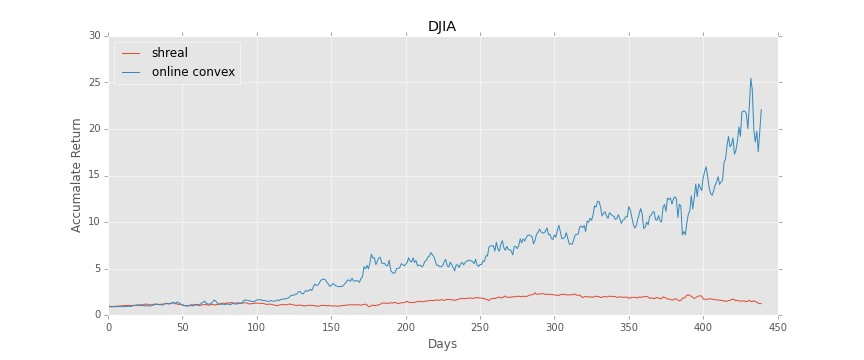
\includegraphics[width=1.0\columnwidth]{DJIA} 
\caption{Cumulative Wealth for SHREAL and Mirror Descent Algorithm on the DJIA Dataset without Transaction Costs.}
\label{DJIA}
\end{figure}

\begin{figure}[!h]
\centering
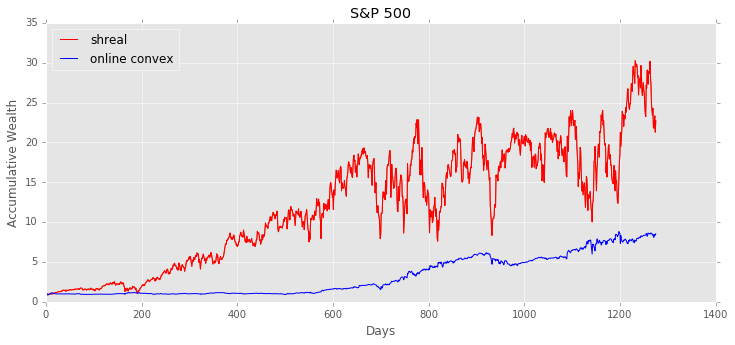
\includegraphics[width=0.85\columnwidth]{S_P500} 
\caption{Cumulative Wealth for SHREAL and Mirror Descent Algorithm on the S\&P 500 Dataset without Transaction Costs.}
\label{S_P500}
\end{figure}

\noindent Figure \ref{DJIA} and Figure \ref{S_P500} illustrate the performances of SHREAL and our Mirror Descent Algorithm on the above mentioned two datasets. The red line represents the results for the benchmark algorithm SHREAL and the blue line corresponds to that of our algorithm. It is clear that our algorithm outperforms SHREAL significantly under the poor market setting, where the accumulative wealth climbed steadily to more than 20 at the end of the 2-year period. The advantage of our algorithm in a good market scenario, where only a few stocks lost value, is less obvious. As shown in Figure \ref{S_P500}, although SHREAL achieved a higher return, its large and frequent fluctuations indicate higher risk compared with the stable growing pattern demonstrated by the Mirror Descent Algorithm. Results from both datasets show that our Mirror Descent Algorithm does a better risk control while giving desired return. 

\subsection{Manipulation of Parameters}

\begin{figure}[!h]
\centering
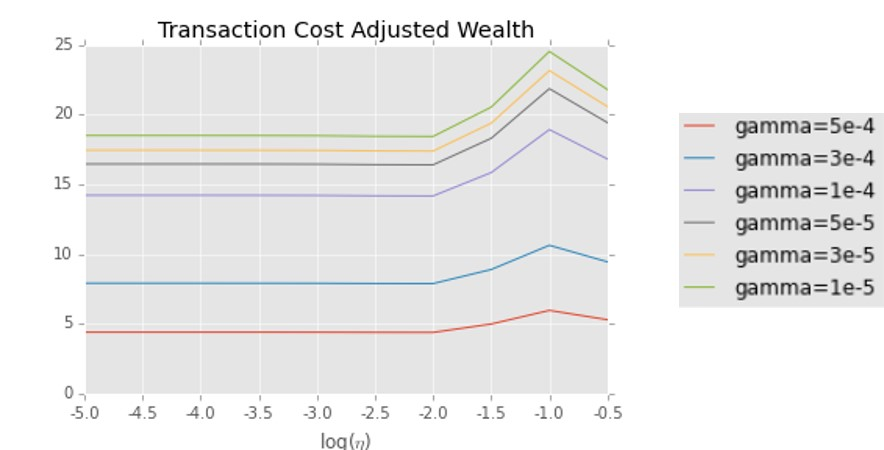
\includegraphics[width=0.85\columnwidth]{para} 
\caption{Cumulative Wealth for Mirror Descent Algorithm on the DJIA with Different transaction costs.}
\label{S_P500}
\end{figure}

\section{Conclusion}
In this project, we propose a Mirror Descent algorithm for online portfolio selection which takes into consideration of both leveraging and hedging. Moreover, we have added regularization terms for mean reversion theory and price momentum which better fit the market. Our experimental results shows that this Mirror Descent Algorithm provides strategies which can effectively control exposure to risk and lead to competitive return. It especially outperforms the SHREAL algorithm, which has been proven better than many state-of-the-art portfolio selection algorithms, in poor market.

\bibliographystyle{IEEEtran}
\bibliography{references_227}
\end{document} to your LaTeX file where you want your
% title page.
%
%%%%%%%%%%%%%%%%%%%%%%%%%%%%%%%%%%%%%%%%%
%\title{Title page with logo}
%----------------------------------------------------------------------------------------
%	PACKAGES AND OTHER DOCUMENT CONFIGURATIONS
%----------------------------------------------------------------------------------------

\documentclass[12pt]{article}
\usepackage[english]{babel}
\usepackage[utf8x]{inputenc}
\usepackage{amsmath}
\usepackage{graphicx}
\usepackage[colorinlistoftodos]{todonotes}
\usepackage{setspace}
\usepackage{algpseudocode}
\usepackage{algorithm}
\usepackage{amsthm} \usepackage{color, colortbl}
\usepackage{cite}
\begin{document}

\begin{titlepage}

\newcommand{\HRule}{\rule{\linewidth}{0.5mm}} % Defines a new command for the horizontal lines, change thickness here

\center % Center everything on the page
 
%----------------------------------------------------------------------------------------
%	HEADING SECTIONS
%----------------------------------------------------------------------------------------

\textsc{\LARGE EECS 227C}\\[1.0cm] % Name of your university/college
\textsc{\Large Course Project}\\[2.0cm] % Major heading such as course name

%----------------------------------------------------------------------------------------
%	TITLE SECTION
%----------------------------------------------------------------------------------------

% \HRule \\[0.3cm]
\singlespacing \huge \textbf{Mirror Descent Method for Online Portfolio Allocation with Hedging}
\\[0.2cm] % Title of your document
\HRule \\[2.0cm]
 
%----------------------------------------------------------------------------------------
%	AUTHOR SECTION
%----------------------------------------------------------------------------------------

\begin{minipage}{0.4\textwidth}
\begin{flushleft} \large
\emph{Name:}\\
Ying \textsc{Cao}\\
Shiman \textsc{Ding}\\
Renyuan \textsc{Xu}
\end{flushleft}
\end{minipage}
~
\begin{minipage}{0.4\textwidth}
\begin{flushright} \large
\emph{SID:} \\
25937400\\
24104985\\
25945145
\end{flushright}
\end{minipage}\\[2.5cm]

% If you don't want a supervisor, uncomment the two lines below and remove the section above
%\Large \emph{Author:}\\
%John \textsc{Smith}\\[3cm] % Your name

%----------------------------------------------------------------------------------------
%	DATE SECTION
%----------------------------------------------------------------------------------------

{\large \today}\\[2cm] % Date, change the \today to a set date if you want to be precise

%----------------------------------------------------------------------------------------
%	LOGO SECTION
%----------------------------------------------------------------------------------------

% \includegraphics{logo.png}\\[1cm] % Include a department/university logo - this will require the graphicx package
 
%----------------------------------------------------------------------------------------

\vfill % Fill the rest of the page with whitespace

\end{titlepage}

\onehalfspacing
\begin{abstract}
Online portfolio selection is a fundamental problem in computational finance, which has been extensively studied across several research communities, including finance, statistics, artificial intelligence, machine learning, and data mining, etc.
In this project we incorporate structured hedging, price mean reversion, and other loss penalty terms into the model of portfolio management. We present a formulation for hedging online resource allocations with leverage and propose mirror descent method to solve the problem sequentially. We implement our model on SP500 and DJIA dataset, and compare our algorithm with a recently proposed algorithm, SHREAL, by \cite{johnson2015structured} to see the difference.
\end{abstract}


\section{Introduction}

Online resource allocation is a fundamental problem problem in mathematical finance. It is complicated since the optimal portfolio selection
strategy should take into consideration not only maximizing the expected return, but also the risk management of the portfolio. And it becomes a more challenging problem when we allow for leveraging and transaction costs.\\

\noindent Previous research \cite{johnson2015online,blum1999universal,kalai2003efficient} has been focusing extensively on portfolio management under limited budget. That is, they only consider strategies with resources on hand. But in reality, especially in stock market, people can borrow additional money at certain risk to apply leverage and increase return. Such leverage provides us more flexibility in management, as well as more risk since profits and losses are all magnified. One common method to control risk is to hedge. Specifically for stock markets, stocks are more often correlated than independent. Taking advantage of these correlations, we can invest in the same or opposite directions in different stocks to hedge risk. For example, HSBA-LN and HSBC are two stocks based on the same underlying company, hence their returns are highly correlated. Then if we long position in one and short position in the other, the risk is almost perfectly hedged, which protects our investment if market crashes.\\

\noindent In this paper, we incorporate different regularization terms into portfolio management, including a correlation graph of hedging, price mean reversion and momentum regularization, loss function for profits and losses. We also analyze our algorithm under different transaction costs on different datasets.

\section{Precursors}
\subsection{Long and Short Positions}
For each stock, we can hold two positions: long and short. A \textbf{long position} means we buy the stock with our money on hand, and if the stock price goes up, we make some profit. In contrast, a \textbf{short position} is taken when we borrowed some stock and sell on the market. And one will profit if its price decreases. In this paper, we assume both long and short positions can be taken at any number of shares.

\subsection{Hedging and Leverage}
As we mentioned before, \textbf{hedging} takes advantage of the structural dependencies between the assets and offsets the risk of a particular allocation by utilizing both short and long positions. It is specially important when market crashes. Given any $n$ stocks, We build a correlation graph of $2n$ nodes and $2n\cdot n$ edges, where each stock is associated with two nodes, one for long position and one for short position. The graph is bipartite with natural partition of long and short positions. An edge is made between any two nodes with opposite positions and the weight of the edge is the correlation of the two stocks of the nodes (could be the same). If two stocks are highly positive correlated, we want our portfolio to take opposite directions in them so as to lower risk in the portfolio.\\ 

\noindent \textbf{Leverage} is another useful tool in financial  market, where we borrow money from some external resource, say bank, to increase allocation power. It helps to amply the potential return at the cost of exposure to higher risk in our investment. A common practice in stock market is to buy on margins. This is to buy stocks using cash borrowed, and is usually operated by putting some money into a margin account. Interest is also charged on the loan.

\subsection{Mean Reversion}
Price change of a stock reflects market's view on its fair value. Price goes up if the current price is under people's expectation and vice versa. But in many scenarios, market tends to overreact to news or other event occurring in the market. That is also intuitive to what we observe in daily life, when the price of a stock goes up dramatically, it is more like to decrease next day, which is called \textbf{mean reversion} phenomenon of stock price. Extensive studies, such as \cite{li2012line}, have shown that mean reversion strategies may better fit the market and give better empirical results. This inspires us to includes a regulation term to  capture this property in our formulation.

\subsection{Price Momentum }
\textbf{Price momentum} is the opposite action of mean reversion property. The idea behind this theory is simple that investors will buy past winners and sell past losers so that price is more likely to keep moving in the same direction than to change directions. This theory helps lower noises and smooth our management of portfolio. It is specially useful when traders want to execute huge volume while minimize price impact on the market. 


\section{Problem Formulation}
In this section, we introduce a framework adopted from [1] for structured hedging with leverage, and consider the online resource allocation problem under such structured hedging.

\subsection{Some Notations}
    \noindent For any $n$ stocks, our goal is to find an allocation $p \in P \subset R^{2n}$ which determines how to split up a resource among long and short positions over the $n$ stocks such that a certain loss function $f(p)$ is minimized. Denote the set of of index $l=\{1,...,n\}$ and $s=\{n+1, n+2, ... 2n\}$ as the long and short positions in $p$ and let $D_l$ and $D_s$ be $2n$ by $2n$ diagonal matrix with $D_l(i,i)=1, \forall i\in l$, $D_s(i,i)=1, \forall i\in s$. Let $q_l = D_lp \geq 0, q_s = D_sp \leq
    0$, in which $q_l \geq 0$ and $q_s \leq 0$ is the long only and short only vectors. The basic idea for hedging is place money in opposing positions and different assets. We can make use of the structural dependencies between stocks to effectively control risk by constructing a correlation Matrix $W$ as discussed above.\\

    \noindent We consider a stock market consisting of $n$ stocks $\{s_1,...s_n\}$ over $T$ periods. In our numerical experiments, we consider a period to be a day, but same analysis holds for any other valid period definition. Let $x_t(i)$ denote the \textbf{price relative} of stock $s_i$ in day $t$, which is the ratio of current price over previous price. Clearly, $x_t(i) > 1$ means an increase in price, and $x_t(i) < 1$ means a decrease in price. Let 
    $\hat{x_t} = [x_t(1),...x_t(n)]^T$ denote the vector of price relatives for day $t$. For the convenience of formulation, we denote $x_t = [\hat{x_t}, \hat{x_t}]^T$. The portfolio on day $t$ is $p_t = [p_t(1),...p_t(2n)]^T$, in which the first $l$ positions are for long-only allocation, and the last $s$ positions are for short-only allocation.\\

    \noindent Assume bank interest is $r$ per day. At the end of the day $t$, the multiplicative gain in wealth is :
    $$\phi (t) = q_l^Tx_t + (1-q_l^T\textbf{1})(1+r) + q_s^T(x_t-1+r)$$
    in which the first item is the gain from long position, the second item is the gain or loss from saving or leverage, and the third item is the gain from short positions. We assume the change in price are bounded as $ 0 < 1 - B_l < x_t < 1 + B_s < \infty$ to guarantee the positiveness of this multiplicative gain. Therefore, we can put constrains $q_l \geq 0, q_s \leq 0, a^Tp \leq \frac{1+r}{r+B_l}$ on $p$ to ensure we are not going to have negative wealth at the end of a day after selling out all stocks and paying back money borrowed from bank. In the constraints, according to \cite{johnson2015structured}, for vector $a$, we set the first $l$ elements are equal to 1 and the last $s$ elements are equal to $-\frac{B_s+r}{B_l+r}$.\\ 


\subsection{Loss functions}

    \noindent In order to formulate the portfolio management problem as an online convex optimization. We first need to define a loss function for day $t$. Our loss function consists four parts:
    $$l_t(p) = \xi l_t^{0}(p) + \lambda l_t^{d}(p) + \alpha l_t^{r}(p) + \beta l_t^{m}(p)$$

    \begin{itemize}

        \item The first term $l_t^0(p)$ is the negative logrithm of the multiplicative gain of day $t$.
            $$l_t^{0}(p) = -log(a_1q_l^Tx_t + a_2q_s^T(x_t-1+r) + (1-q_l^T\textbf{1})(1+r))$$
            in which $a_1, a_2$ are the weights put on long positions and short positions respectively to control their importance.\\

        \item The second term $l_t^d(p)$ is the hedging penalty function based on estimated structural dependencies.
            $$l_t^{d}(p) = \sum_{i=1}^n\sum_{j=1+n, j\neq i+n}^{2n} Corr(i,j)(q_l(i)+q_s(j))^2$$
            in which $Corr(i,j)$ is the estimated correlation between stock $i$ and $j$ based on historical data from the previous $\delta$ days. When $Corr(i,j)$ is large, we minimize this loss by making the opposing positions of $i,j$ close. This minimization can effectively encourage hedging. This loss term can be rewritten in the following matrix form:
            $$l_t^{d}(p) = p^TLp$$
            in which $L=U+D$, $U = [0, W; W, 0]$. $W$ is the estimated correlation matrix, $D$ is a diagonal matrix with $D(i,i)=\sum_j U(i,j)$.

        \item The third term $l_t^r(p)$ is the mean reversion penalty based on the the mean reversion theory.
            $$l_t^r(p)=(x_{t} - 1)^Tp$$

        \item Finally, the fourth term $l_t^m(p_t)$ is the momentum penalty:
            $$l_t^m(p)=\frac{1}{2}||p-2p_{t}+p_{t-1})||^2$$

    \end{itemize}


    \noindent Clearly, this loss function is convex, take the derivative of $l_t(p)$, we have:
\begin{align}\nonumber
\nabla l_t(p) & = \xi \frac{\alpha_1D_l^Tx_t+\alpha_2D_s^T(x_t-1+r)-D_l^T\textbf{1}(1+r)}{\alpha_1p^TD_l^Tx_t+\alpha_2p^TD_s^T(x_t-1+r)+(1-p^TD_l^T\textbf{1})(1+r)} \\ &\  \ + \lambda (L^T+L)p + \alpha (x_{t}-1) + \beta (p - 2p_{t} + p_{t-1})
\end{align}

\subsection{Regularized linear game}

    By a first-order Taylor expansion of the defined lodd function $\_t$ at $p_t$, we formulate the portfolio selection problem as follows:

    \begin{align} \label{1}
    p_{t+1} = argmin_{q_l \geq 0, q_s \leq 0, a^Tp\leq \frac{1+r}{B_l+r}} \bigg\{\eta_t \nabla l_t(p_t)^Tp + \frac{1}{2}||p-p_t||_2^2\bigg\} 
    \end{align}
    \noindent Since $l_t(p)$ is strongly convex, we can use mirror descent with a step size of $O(\frac{1}{t})$ to ensure a regret bound of $O(log T)$. That is,

    $$\hat{L}_n - L_n^{\star} \leq O(log T)$$

\section{Mirror Descent Algorithm}

    \begin{algorithm}
        \caption{Proposed Algorithm for Structural Hedging}
        \begin{algorithmic}
            \State $\xi, \alpha_1, \alpha_2, \lambda, \alpha, \beta, B_l, B_s, r$, transiction cost $\gamma$, days lag $\delta$, step size decay factor $r$
            \State $S_0 \leftarrow 1, p_0 \leftarrow 0$
            \For  {$t=1$ to $T$} 
            \State Observe the relative price $\bf{x_t}$ 
            \State Compute multiplicative gain $\phi_t$
            \State Compute total wealth : $S_{t} = S_{t-1}(\phi_t-\gamma||p_t-p_{t-1}||_1)$
            \If{$t \leq \delta$}
            \State $p_t \leftarrow p_{t-1}$
            \Else
            \State Update correlation matrix $W$: $W_{ij} \leftarrow \frac{\sum\limits_{k=1}^t x_k^i\cdot \sum\limits_{k=1}^t x_k^j - \sum\limits_{k=1}^t x_k^ix_k^j}{var(\bf{x^i})\cdot var(\bf{x^j})}$
            \State $\eta_t \leftarrow \frac{1}{1 + rt}$
            \State $p_{t+1} = \Pi_P (\nabla R^{-1}(\nabla R(p_t) - \eta_t \nabla l_t(p_t)))$
            \EndIf  
            \EndFor 
        \end{algorithmic}
    \end{algorithm}
where $\Pi_P(x)$ is a projection to space $P$.
For each day, a correlation matrix is estimated using price relatives from the previous $\delta$ days, parameter $\eta$ is updated, and final a new allocation strategy $p_{t+1}$ is obtained by solving (\ref{1}), and $R$ is the identity mapping. 

\section{Numerical Results}

\subsection{Datasets}
The experiments were conducted on 2 datasets with data taken from Dow Jones Industrial Average (DJIA) and Standard \& Poor's 500 (S\&P 500). These two datasets are freely available online and have been widely used in numerous empirical studies in the field of computational finance, thus make our numerical results comparable to those from many classical algorithms (may refer to \cite{johnson2015structured,das2014online}).\\

\noindent The former dataset consists of 30 stocks and 507 trading days over a period of 2 years from 2001 to 2003, and the other consists
of 25 stocks and 1276 trading days over a period of 5 years from 1998 to 2003. They are very different in nature where 83\% stocks in the DJIA lost value while only 28\% stocks in SP500 lost value. Thus, these two datasets are representative for two very distinct markets. And our experiments show that our Mirror Descent Algorithm performs stably well in both of the markets.


\subsection{Implementation of Projection}
To implement the projection step of our algorithm, we first adopt an alternating projections approach as suggested by \cite{johnson2015structured}. This technique works well on both of the datasets within seconds. However, depending on the data, the convergence of the method of alternating projections can be arbitrarily slow. To overcome this shortcoming, we switched to direct projecting to simplex. 

\subsection{Comparison with SHREAL}
SHREAL is an online portfolio selection algorithm proposed by Johnson et al in \cite{johnson2015structured}, which also take accounts hedging and leveraging. It is also shown that SHREAL outperforms many classical algorithms and thus, we used SHREAL as a benchmark algorithm. To evaluate the practical application of our Mirror Descent Algorithm, we use cumulative wealth as the metric. Parameters are tuned in sample such that maximum cumulative wealth (without transaction costs) can be achieved. It is latter showed that stable behavior can be found even if we perturb the parameters. Moreover, this algorithm can also incorporate transaction costs by setting none-zero value for $\gamma$.

\begin{figure}[!h]
\centering
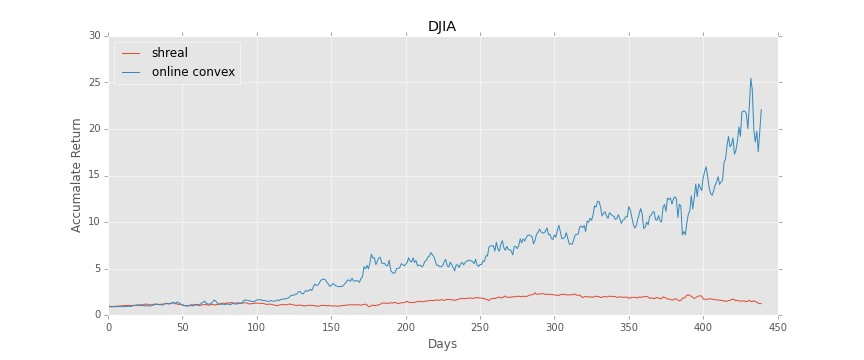
\includegraphics[width=1.0\columnwidth]{DJIA} 
\caption{Cumulative Wealth for SHREAL and Mirror Descent Algorithm on the DJIA Dataset without Transaction Costs.}
\label{DJIA}
\end{figure}

\begin{figure}[!h]
\centering
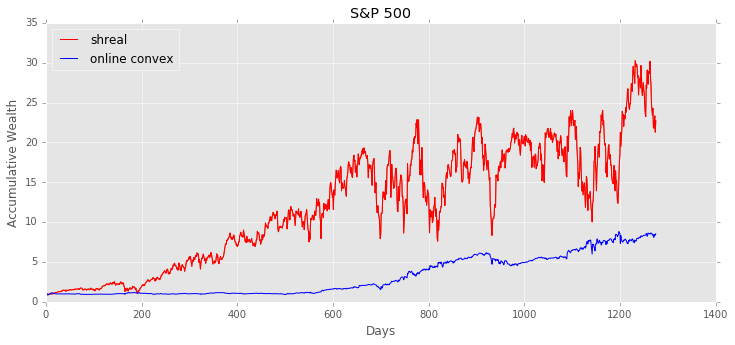
\includegraphics[width=0.85\columnwidth]{S_P500} 
\caption{Cumulative Wealth for SHREAL and Mirror Descent Algorithm on the S\&P 500 Dataset without Transaction Costs.}
\label{S_P500}
\end{figure}

\noindent Figure \ref{DJIA} and Figure \ref{S_P500} illustrate the performances of SHREAL and our Mirror Descent Algorithm on the above mentioned two datasets. The red line represents the results for the benchmark algorithm SHREAL and the blue line corresponds to that of our algorithm. It is clear that our algorithm outperforms SHREAL significantly under the poor market setting, where the accumulative wealth climbed steadily to more than 20 at the end of the 2-year period. The advantage of our algorithm in a good market scenario, where only a few stocks lost value, is less obvious. As shown in Figure \ref{S_P500}, although SHREAL achieved a higher return, its large and frequent fluctuations indicate higher risk compared with the stable growing pattern demonstrated by the Mirror Descent Algorithm. Results from both datasets show that our Mirror Descent Algorithm does a better risk control while giving desired return. 

\subsection{Manipulation of Parameters}

\begin{figure}[!h]
\centering
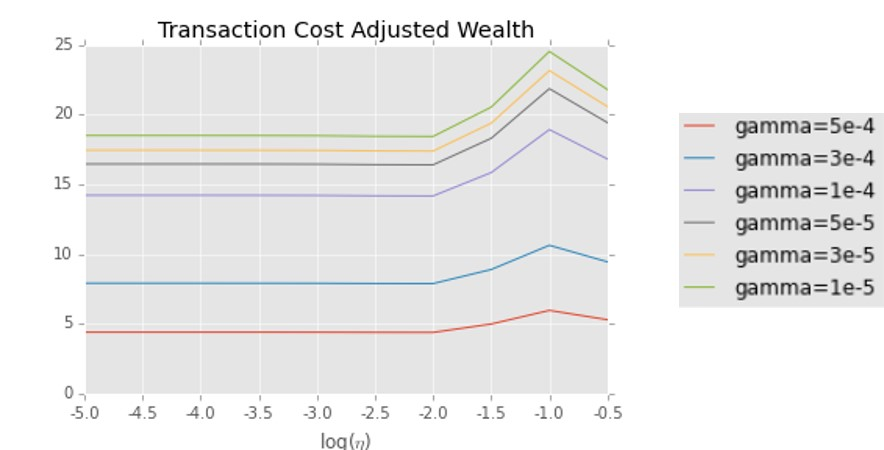
\includegraphics[width=0.85\columnwidth]{para} 
\caption{Cumulative Wealth for Mirror Descent Algorithm on the DJIA with Different transaction costs.}
\label{S_P500}
\end{figure}

\section{Conclusion}
In this project, we propose a Mirror Descent algorithm for online portfolio selection which takes into consideration of both leveraging and hedging. Moreover, we have added regularization terms for mean reversion theory and price momentum which better fit the market. Our experimental results shows that this Mirror Descent Algorithm provides strategies which can effectively control exposure to risk and lead to competitive return. It especially outperforms the SHREAL algorithm, which has been proven better than many state-of-the-art portfolio selection algorithms, in poor market.

\bibliographystyle{IEEEtran}
\bibliography{references_227}
\end{document} to your LaTeX file where you want your
% title page.
%
%%%%%%%%%%%%%%%%%%%%%%%%%%%%%%%%%%%%%%%%%
%\title{Title page with logo}
%----------------------------------------------------------------------------------------
%	PACKAGES AND OTHER DOCUMENT CONFIGURATIONS
%----------------------------------------------------------------------------------------

\documentclass[12pt]{article}
\usepackage[english]{babel}
\usepackage[utf8x]{inputenc}
\usepackage{amsmath}
\usepackage{graphicx}
\usepackage[colorinlistoftodos]{todonotes}
\usepackage{setspace}
\usepackage{algpseudocode}
\usepackage{algorithm}
\usepackage{amsthm} \usepackage{color, colortbl}
\usepackage{cite}
\begin{document}

\begin{titlepage}

\newcommand{\HRule}{\rule{\linewidth}{0.5mm}} % Defines a new command for the horizontal lines, change thickness here

\center % Center everything on the page
 
%----------------------------------------------------------------------------------------
%	HEADING SECTIONS
%----------------------------------------------------------------------------------------

\textsc{\LARGE EECS 227C}\\[1.0cm] % Name of your university/college
\textsc{\Large Course Project}\\[2.0cm] % Major heading such as course name

%----------------------------------------------------------------------------------------
%	TITLE SECTION
%----------------------------------------------------------------------------------------

% \HRule \\[0.3cm]
\singlespacing \huge \textbf{Mirror Descent Method for Online Portfolio Allocation with Hedging}
\\[0.2cm] % Title of your document
\HRule \\[2.0cm]
 
%----------------------------------------------------------------------------------------
%	AUTHOR SECTION
%----------------------------------------------------------------------------------------

\begin{minipage}{0.4\textwidth}
\begin{flushleft} \large
\emph{Name:}\\
Ying \textsc{Cao}\\
Shiman \textsc{Ding}\\
Renyuan \textsc{Xu}
\end{flushleft}
\end{minipage}
~
\begin{minipage}{0.4\textwidth}
\begin{flushright} \large
\emph{SID:} \\
25937400\\
24104985\\
25945145
\end{flushright}
\end{minipage}\\[2.5cm]

% If you don't want a supervisor, uncomment the two lines below and remove the section above
%\Large \emph{Author:}\\
%John \textsc{Smith}\\[3cm] % Your name

%----------------------------------------------------------------------------------------
%	DATE SECTION
%----------------------------------------------------------------------------------------

{\large \today}\\[2cm] % Date, change the \today to a set date if you want to be precise

%----------------------------------------------------------------------------------------
%	LOGO SECTION
%----------------------------------------------------------------------------------------

% \includegraphics{logo.png}\\[1cm] % Include a department/university logo - this will require the graphicx package
 
%----------------------------------------------------------------------------------------

\vfill % Fill the rest of the page with whitespace

\end{titlepage}

\onehalfspacing
\begin{abstract}
Online portfolio selection is a fundamental problem in computational finance, which has been extensively studied across several research communities, including finance, statistics, artificial intelligence, machine learning, and data mining, etc.
In this project we incorporate structured hedging, price mean reversion, and other loss penalty terms into the model of portfolio management. We present a formulation for hedging online resource allocations with leverage and propose mirror descent method to solve the problem sequentially. We implement our model on SP500 and DJIA dataset, and compare our algorithm with a recently proposed algorithm, SHREAL, by \cite{johnson2015structured} to see the difference.
\end{abstract}


\section{Introduction}

Online resource allocation is a fundamental problem problem in mathematical finance. It is complicated since the optimal portfolio selection
strategy should take into consideration not only maximizing the expected return, but also the risk management of the portfolio. And it becomes a more challenging problem when we allow for leveraging and transaction costs.\\

\noindent Previous research \cite{johnson2015online,blum1999universal,kalai2003efficient} has been focusing extensively on portfolio management under limited budget. That is, they only consider strategies with resources on hand. But in reality, especially in stock market, people can borrow additional money at certain risk to apply leverage and increase return. Such leverage provides us more flexibility in management, as well as more risk since profits and losses are all magnified. One common method to control risk is to hedge. Specifically for stock markets, stocks are more often correlated than independent. Taking advantage of these correlations, we can invest in the same or opposite directions in different stocks to hedge risk. For example, HSBA-LN and HSBC are two stocks based on the same underlying company, hence their returns are highly correlated. Then if we long position in one and short position in the other, the risk is almost perfectly hedged, which protects our investment if market crashes.\\

\noindent In this paper, we incorporate different regularization terms into portfolio management, including a correlation graph of hedging, price mean reversion and momentum regularization, loss function for profits and losses. We also analyze our algorithm under different transaction costs on different datasets.

\section{Precursors}
\subsection{Long and Short Positions}
For each stock, we can hold two positions: long and short. A \textbf{long position} means we buy the stock with our money on hand, and if the stock price goes up, we make some profit. In contrast, a \textbf{short position} is taken when we borrowed some stock and sell on the market. And one will profit if its price decreases. In this paper, we assume both long and short positions can be taken at any number of shares.

\subsection{Hedging and Leverage}
As we mentioned before, \textbf{hedging} takes advantage of the structural dependencies between the assets and offsets the risk of a particular allocation by utilizing both short and long positions. It is specially important when market crashes. Given any $n$ stocks, We build a correlation graph of $2n$ nodes and $2n\cdot n$ edges, where each stock is associated with two nodes, one for long position and one for short position. The graph is bipartite with natural partition of long and short positions. An edge is made between any two nodes with opposite positions and the weight of the edge is the correlation of the two stocks of the nodes (could be the same). If two stocks are highly positive correlated, we want our portfolio to take opposite directions in them so as to lower risk in the portfolio.\\ 

\noindent \textbf{Leverage} is another useful tool in financial  market, where we borrow money from some external resource, say bank, to increase allocation power. It helps to amply the potential return at the cost of exposure to higher risk in our investment. A common practice in stock market is to buy on margins. This is to buy stocks using cash borrowed, and is usually operated by putting some money into a margin account. Interest is also charged on the loan.

\subsection{Mean Reversion}
Price change of a stock reflects market's view on its fair value. Price goes up if the current price is under people's expectation and vice versa. But in many scenarios, market tends to overreact to news or other event occurring in the market. That is also intuitive to what we observe in daily life, when the price of a stock goes up dramatically, it is more like to decrease next day, which is called \textbf{mean reversion} phenomenon of stock price. Extensive studies, such as \cite{li2012line}, have shown that mean reversion strategies may better fit the market and give better empirical results. This inspires us to includes a regulation term to  capture this property in our formulation.

\subsection{Price Momentum }
\textbf{Price momentum} is the opposite action of mean reversion property. The idea behind this theory is simple that investors will buy past winners and sell past losers so that price is more likely to keep moving in the same direction than to change directions. This theory helps lower noises and smooth our management of portfolio. It is specially useful when traders want to execute huge volume while minimize price impact on the market. 


\section{Problem Formulation}
In this section, we introduce a framework adopted from [1] for structured hedging with leverage, and consider the online resource allocation problem under such structured hedging.

\subsection{Some Notations}
    \noindent For any $n$ stocks, our goal is to find an allocation $p \in P \subset R^{2n}$ which determines how to split up a resource among long and short positions over the $n$ stocks such that a certain loss function $f(p)$ is minimized. Denote the set of of index $l=\{1,...,n\}$ and $s=\{n+1, n+2, ... 2n\}$ as the long and short positions in $p$ and let $D_l$ and $D_s$ be $2n$ by $2n$ diagonal matrix with $D_l(i,i)=1, \forall i\in l$, $D_s(i,i)=1, \forall i\in s$. Let $q_l = D_lp \geq 0, q_s = D_sp \leq
    0$, in which $q_l \geq 0$ and $q_s \leq 0$ is the long only and short only vectors. The basic idea for hedging is place money in opposing positions and different assets. We can make use of the structural dependencies between stocks to effectively control risk by constructing a correlation Matrix $W$ as discussed above.\\

    \noindent We consider a stock market consisting of $n$ stocks $\{s_1,...s_n\}$ over $T$ periods. In our numerical experiments, we consider a period to be a day, but same analysis holds for any other valid period definition. Let $x_t(i)$ denote the \textbf{price relative} of stock $s_i$ in day $t$, which is the ratio of current price over previous price. Clearly, $x_t(i) > 1$ means an increase in price, and $x_t(i) < 1$ means a decrease in price. Let 
    $\hat{x_t} = [x_t(1),...x_t(n)]^T$ denote the vector of price relatives for day $t$. For the convenience of formulation, we denote $x_t = [\hat{x_t}, \hat{x_t}]^T$. The portfolio on day $t$ is $p_t = [p_t(1),...p_t(2n)]^T$, in which the first $l$ positions are for long-only allocation, and the last $s$ positions are for short-only allocation.\\

    \noindent Assume bank interest is $r$ per day. At the end of the day $t$, the multiplicative gain in wealth is :
    $$\phi (t) = q_l^Tx_t + (1-q_l^T\textbf{1})(1+r) + q_s^T(x_t-1+r)$$
    in which the first item is the gain from long position, the second item is the gain or loss from saving or leverage, and the third item is the gain from short positions. We assume the change in price are bounded as $ 0 < 1 - B_l < x_t < 1 + B_s < \infty$ to guarantee the positiveness of this multiplicative gain. Therefore, we can put constrains $q_l \geq 0, q_s \leq 0, a^Tp \leq \frac{1+r}{r+B_l}$ on $p$ to ensure we are not going to have negative wealth at the end of a day after selling out all stocks and paying back money borrowed from bank. In the constraints, according to \cite{johnson2015structured}, for vector $a$, we set the first $l$ elements are equal to 1 and the last $s$ elements are equal to $-\frac{B_s+r}{B_l+r}$.\\ 


\subsection{Loss functions}

    \noindent In order to formulate the portfolio management problem as an online convex optimization. We first need to define a loss function for day $t$. Our loss function consists four parts:
    $$l_t(p) = \xi l_t^{0}(p) + \lambda l_t^{d}(p) + \alpha l_t^{r}(p) + \beta l_t^{m}(p)$$

    \begin{itemize}

        \item The first term $l_t^0(p)$ is the negative logrithm of the multiplicative gain of day $t$.
            $$l_t^{0}(p) = -log(a_1q_l^Tx_t + a_2q_s^T(x_t-1+r) + (1-q_l^T\textbf{1})(1+r))$$
            in which $a_1, a_2$ are the weights put on long positions and short positions respectively to control their importance.\\

        \item The second term $l_t^d(p)$ is the hedging penalty function based on estimated structural dependencies.
            $$l_t^{d}(p) = \sum_{i=1}^n\sum_{j=1+n, j\neq i+n}^{2n} Corr(i,j)(q_l(i)+q_s(j))^2$$
            in which $Corr(i,j)$ is the estimated correlation between stock $i$ and $j$ based on historical data from the previous $\delta$ days. When $Corr(i,j)$ is large, we minimize this loss by making the opposing positions of $i,j$ close. This minimization can effectively encourage hedging. This loss term can be rewritten in the following matrix form:
            $$l_t^{d}(p) = p^TLp$$
            in which $L=U+D$, $U = [0, W; W, 0]$. $W$ is the estimated correlation matrix, $D$ is a diagonal matrix with $D(i,i)=\sum_j U(i,j)$.

        \item The third term $l_t^r(p)$ is the mean reversion penalty based on the the mean reversion theory.
            $$l_t^r(p)=(x_{t} - 1)^Tp$$

        \item Finally, the fourth term $l_t^m(p_t)$ is the momentum penalty:
            $$l_t^m(p)=\frac{1}{2}||p-2p_{t}+p_{t-1})||^2$$

    \end{itemize}


    \noindent Clearly, this loss function is convex, take the derivative of $l_t(p)$, we have:
\begin{align}\nonumber
\nabla l_t(p) & = \xi \frac{\alpha_1D_l^Tx_t+\alpha_2D_s^T(x_t-1+r)-D_l^T\textbf{1}(1+r)}{\alpha_1p^TD_l^Tx_t+\alpha_2p^TD_s^T(x_t-1+r)+(1-p^TD_l^T\textbf{1})(1+r)} \\ &\  \ + \lambda (L^T+L)p + \alpha (x_{t}-1) + \beta (p - 2p_{t} + p_{t-1})
\end{align}

\subsection{Regularized linear game}

    By a first-order Taylor expansion of the defined lodd function $\_t$ at $p_t$, we formulate the portfolio selection problem as follows:

    \begin{align} \label{1}
    p_{t+1} = argmin_{q_l \geq 0, q_s \leq 0, a^Tp\leq \frac{1+r}{B_l+r}} \bigg\{\eta_t \nabla l_t(p_t)^Tp + \frac{1}{2}||p-p_t||_2^2\bigg\} 
    \end{align}
    \noindent Since $l_t(p)$ is strongly convex, we can use mirror descent with a step size of $O(\frac{1}{t})$ to ensure a regret bound of $O(log T)$. That is,

    $$\hat{L}_n - L_n^{\star} \leq O(log T)$$

\section{Mirror Descent Algorithm}

    \begin{algorithm}
        \caption{Proposed Algorithm for Structural Hedging}
        \begin{algorithmic}
            \State $\xi, \alpha_1, \alpha_2, \lambda, \alpha, \beta, B_l, B_s, r$, transiction cost $\gamma$, days lag $\delta$, step size decay factor $r$
            \State $S_0 \leftarrow 1, p_0 \leftarrow 0$
            \For  {$t=1$ to $T$} 
            \State Observe the relative price $\bf{x_t}$ 
            \State Compute multiplicative gain $\phi_t$
            \State Compute total wealth : $S_{t} = S_{t-1}(\phi_t-\gamma||p_t-p_{t-1}||_1)$
            \If{$t \leq \delta$}
            \State $p_t \leftarrow p_{t-1}$
            \Else
            \State Update correlation matrix $W$: $W_{ij} \leftarrow \frac{\sum\limits_{k=1}^t x_k^i\cdot \sum\limits_{k=1}^t x_k^j - \sum\limits_{k=1}^t x_k^ix_k^j}{var(\bf{x^i})\cdot var(\bf{x^j})}$
            \State $\eta_t \leftarrow \frac{1}{1 + rt}$
            \State $p_{t+1} = \Pi_P (\nabla R^{-1}(\nabla R(p_t) - \eta_t \nabla l_t(p_t)))$
            \EndIf  
            \EndFor 
        \end{algorithmic}
    \end{algorithm}
where $\Pi_P(x)$ is a projection to space $P$.
For each day, a correlation matrix is estimated using price relatives from the previous $\delta$ days, parameter $\eta$ is updated, and final a new allocation strategy $p_{t+1}$ is obtained by solving (\ref{1}), and $R$ is the identity mapping. 

\section{Numerical Results}

\subsection{Datasets}
The experiments were conducted on 2 datasets with data taken from Dow Jones Industrial Average (DJIA) and Standard \& Poor's 500 (S\&P 500). These two datasets are freely available online and have been widely used in numerous empirical studies in the field of computational finance, thus make our numerical results comparable to those from many classical algorithms (may refer to \cite{johnson2015structured,das2014online}).\\

\noindent The former dataset consists of 30 stocks and 507 trading days over a period of 2 years from 2001 to 2003, and the other consists
of 25 stocks and 1276 trading days over a period of 5 years from 1998 to 2003. They are very different in nature where 83\% stocks in the DJIA lost value while only 28\% stocks in SP500 lost value. Thus, these two datasets are representative for two very distinct markets. And our experiments show that our Mirror Descent Algorithm performs stably well in both of the markets.


\subsection{Implementation of Projection}
To implement the projection step of our algorithm, we first adopt an alternating projections approach as suggested by \cite{johnson2015structured}. This technique works well on both of the datasets within seconds. However, depending on the data, the convergence of the method of alternating projections can be arbitrarily slow. To overcome this shortcoming, we switched to direct projecting to simplex. 

\subsection{Comparison with SHREAL}
SHREAL is an online portfolio selection algorithm proposed by Johnson et al in \cite{johnson2015structured}, which also take accounts hedging and leveraging. It is also shown that SHREAL outperforms many classical algorithms and thus, we used SHREAL as a benchmark algorithm. To evaluate the practical application of our Mirror Descent Algorithm, we use cumulative wealth as the metric. Parameters are tuned in sample such that maximum cumulative wealth (without transaction costs) can be achieved. It is latter showed that stable behavior can be found even if we perturb the parameters. Moreover, this algorithm can also incorporate transaction costs by setting none-zero value for $\gamma$.

\begin{figure}[!h]
\centering
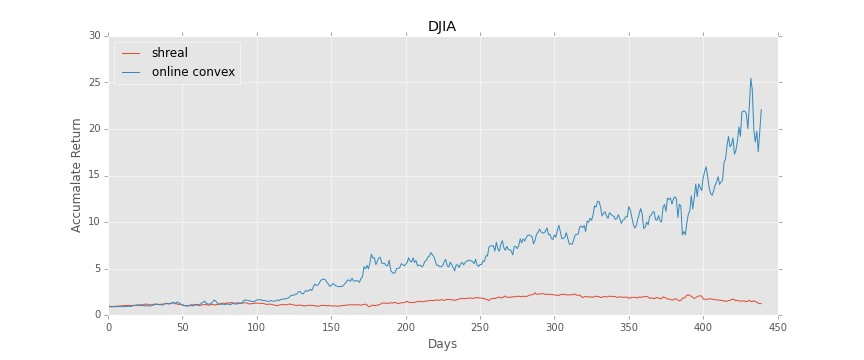
\includegraphics[width=1.0\columnwidth]{DJIA} 
\caption{Cumulative Wealth for SHREAL and Mirror Descent Algorithm on the DJIA Dataset without Transaction Costs.}
\label{DJIA}
\end{figure}

\begin{figure}[!h]
\centering
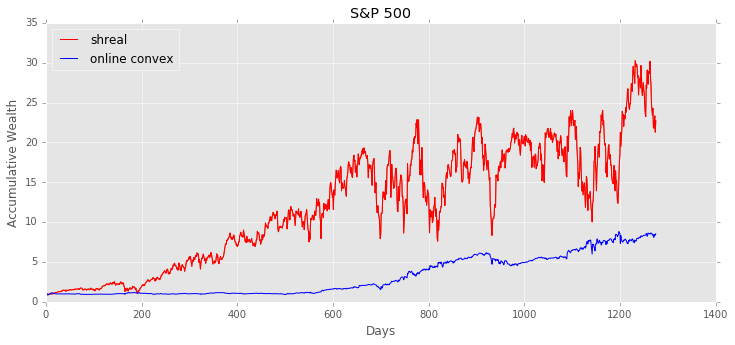
\includegraphics[width=0.85\columnwidth]{S_P500} 
\caption{Cumulative Wealth for SHREAL and Mirror Descent Algorithm on the S\&P 500 Dataset without Transaction Costs.}
\label{S_P500}
\end{figure}

\noindent Figure \ref{DJIA} and Figure \ref{S_P500} illustrate the performances of SHREAL and our Mirror Descent Algorithm on the above mentioned two datasets. The red line represents the results for the benchmark algorithm SHREAL and the blue line corresponds to that of our algorithm. It is clear that our algorithm outperforms SHREAL significantly under the poor market setting, where the accumulative wealth climbed steadily to more than 20 at the end of the 2-year period. The advantage of our algorithm in a good market scenario, where only a few stocks lost value, is less obvious. As shown in Figure \ref{S_P500}, although SHREAL achieved a higher return, its large and frequent fluctuations indicate higher risk compared with the stable growing pattern demonstrated by the Mirror Descent Algorithm. Results from both datasets show that our Mirror Descent Algorithm does a better risk control while giving desired return. 

\subsection{Manipulation of Parameters}

\begin{figure}[!h]
\centering
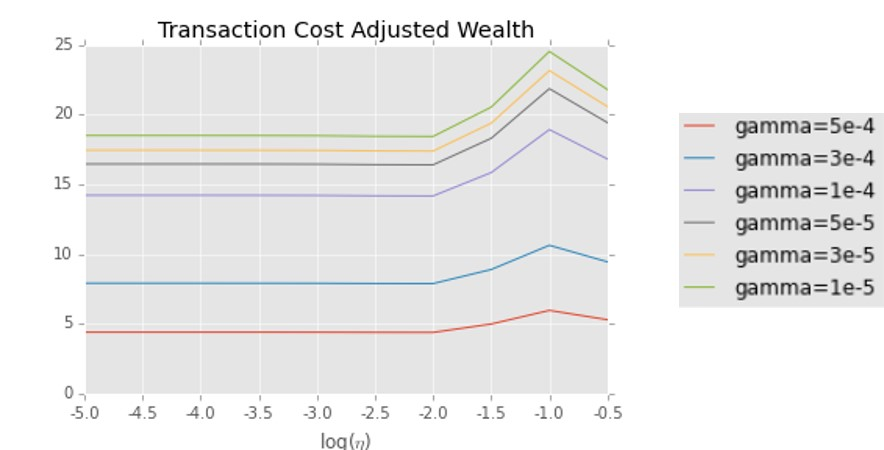
\includegraphics[width=0.85\columnwidth]{para} 
\caption{Cumulative Wealth for Mirror Descent Algorithm on the DJIA with Different transaction costs.}
\label{S_P500}
\end{figure}

\section{Conclusion}
In this project, we propose a Mirror Descent algorithm for online portfolio selection which takes into consideration of both leveraging and hedging. Moreover, we have added regularization terms for mean reversion theory and price momentum which better fit the market. Our experimental results shows that this Mirror Descent Algorithm provides strategies which can effectively control exposure to risk and lead to competitive return. It especially outperforms the SHREAL algorithm, which has been proven better than many state-of-the-art portfolio selection algorithms, in poor market.

\bibliographystyle{IEEEtran}
\bibliography{references_227}
\end{document} to your LaTeX file where you want your
% title page.
%
%%%%%%%%%%%%%%%%%%%%%%%%%%%%%%%%%%%%%%%%%
%\title{Title page with logo}
%----------------------------------------------------------------------------------------
%	PACKAGES AND OTHER DOCUMENT CONFIGURATIONS
%----------------------------------------------------------------------------------------

\documentclass[12pt]{article}
\usepackage[english]{babel}
\usepackage[utf8x]{inputenc}
\usepackage{amsmath}
\usepackage{graphicx}
\usepackage[colorinlistoftodos]{todonotes}
\usepackage{setspace}
\usepackage{algpseudocode}
\usepackage{algorithm}
\usepackage{amsthm} \usepackage{color, colortbl}
\usepackage{cite}
\begin{document}

\begin{titlepage}

\newcommand{\HRule}{\rule{\linewidth}{0.5mm}} % Defines a new command for the horizontal lines, change thickness here

\center % Center everything on the page
 
%----------------------------------------------------------------------------------------
%	HEADING SECTIONS
%----------------------------------------------------------------------------------------

\textsc{\LARGE EECS 227C}\\[1.0cm] % Name of your university/college
\textsc{\Large Course Project}\\[2.0cm] % Major heading such as course name

%----------------------------------------------------------------------------------------
%	TITLE SECTION
%----------------------------------------------------------------------------------------

% \HRule \\[0.3cm]
\singlespacing \huge \textbf{Mirror Descent Method for Online Portfolio Allocation with Hedging}
\\[0.2cm] % Title of your document
\HRule \\[2.0cm]
 
%----------------------------------------------------------------------------------------
%	AUTHOR SECTION
%----------------------------------------------------------------------------------------

\begin{minipage}{0.4\textwidth}
\begin{flushleft} \large
\emph{Name:}\\
Ying \textsc{Cao}\\
Shiman \textsc{Ding}\\
Renyuan \textsc{Xu}
\end{flushleft}
\end{minipage}
~
\begin{minipage}{0.4\textwidth}
\begin{flushright} \large
\emph{SID:} \\
25937400\\
24104985\\
25945145
\end{flushright}
\end{minipage}\\[2.5cm]

% If you don't want a supervisor, uncomment the two lines below and remove the section above
%\Large \emph{Author:}\\
%John \textsc{Smith}\\[3cm] % Your name

%----------------------------------------------------------------------------------------
%	DATE SECTION
%----------------------------------------------------------------------------------------

{\large \today}\\[2cm] % Date, change the \today to a set date if you want to be precise

%----------------------------------------------------------------------------------------
%	LOGO SECTION
%----------------------------------------------------------------------------------------

% \includegraphics{logo.png}\\[1cm] % Include a department/university logo - this will require the graphicx package
 
%----------------------------------------------------------------------------------------

\vfill % Fill the rest of the page with whitespace

\end{titlepage}

\onehalfspacing
\begin{abstract}
Online portfolio selection is a fundamental problem in computational finance, which has been extensively studied across several research communities, including finance, statistics, artificial intelligence, machine learning, and data mining, etc.
In this project we incorporate structured hedging, price mean reversion, and other loss penalty terms into the model of portfolio management. We present a formulation for hedging online resource allocations with leverage and propose mirror descent method to solve the problem sequentially. We implement our model on SP500 and DJIA dataset, and compare our algorithm with a recently proposed algorithm, SHREAL, by \cite{johnson2015structured} to see the difference.
\end{abstract}


\section{Introduction}

Online resource allocation is a fundamental problem problem in mathematical finance. It is complicated since the optimal portfolio selection
strategy should take into consideration not only maximizing the expected return, but also the risk management of the portfolio. And it becomes a more challenging problem when we allow for leveraging and transaction costs.\\

\noindent Previous research \cite{johnson2015online,blum1999universal,kalai2003efficient} has been focusing extensively on portfolio management under limited budget. That is, they only consider strategies with resources on hand. But in reality, especially in stock market, people can borrow additional money at certain risk to apply leverage and increase return. Such leverage provides us more flexibility in management, as well as more risk since profits and losses are all magnified. One common method to control risk is to hedge. Specifically for stock markets, stocks are more often correlated than independent. Taking advantage of these correlations, we can invest in the same or opposite directions in different stocks to hedge risk. For example, HSBA-LN and HSBC are two stocks based on the same underlying company, hence their returns are highly correlated. Then if we long position in one and short position in the other, the risk is almost perfectly hedged, which protects our investment if market crashes.\\

\noindent In this paper, we incorporate different regularization terms into portfolio management, including a correlation graph of hedging, price mean reversion and momentum regularization, loss function for profits and losses. We also analyze our algorithm under different transaction costs on different datasets.

\section{Precursors}
\subsection{Long and Short Positions}
For each stock, we can hold two positions: long and short. A \textbf{long position} means we buy the stock with our money on hand, and if the stock price goes up, we make some profit. In contrast, a \textbf{short position} is taken when we borrowed some stock and sell on the market. And one will profit if its price decreases. In this paper, we assume both long and short positions can be taken at any number of shares.

\subsection{Hedging and Leverage}
As we mentioned before, \textbf{hedging} takes advantage of the structural dependencies between the assets and offsets the risk of a particular allocation by utilizing both short and long positions. It is specially important when market crashes. Given any $n$ stocks, We build a correlation graph of $2n$ nodes and $2n\cdot n$ edges, where each stock is associated with two nodes, one for long position and one for short position. The graph is bipartite with natural partition of long and short positions. An edge is made between any two nodes with opposite positions and the weight of the edge is the correlation of the two stocks of the nodes (could be the same). If two stocks are highly positive correlated, we want our portfolio to take opposite directions in them so as to lower risk in the portfolio.\\ 

\noindent \textbf{Leverage} is another useful tool in financial  market, where we borrow money from some external resource, say bank, to increase allocation power. It helps to amply the potential return at the cost of exposure to higher risk in our investment. A common practice in stock market is to buy on margins. This is to buy stocks using cash borrowed, and is usually operated by putting some money into a margin account. Interest is also charged on the loan.

\subsection{Mean Reversion}
Price change of a stock reflects market's view on its fair value. Price goes up if the current price is under people's expectation and vice versa. But in many scenarios, market tends to overreact to news or other event occurring in the market. That is also intuitive to what we observe in daily life, when the price of a stock goes up dramatically, it is more like to decrease next day, which is called \textbf{mean reversion} phenomenon of stock price. Extensive studies, such as \cite{li2012line}, have shown that mean reversion strategies may better fit the market and give better empirical results. This inspires us to includes a regulation term to  capture this property in our formulation.

\subsection{Price Momentum }
\textbf{Price momentum} is the opposite action of mean reversion property. The idea behind this theory is simple that investors will buy past winners and sell past losers so that price is more likely to keep moving in the same direction than to change directions. This theory helps lower noises and smooth our management of portfolio. It is specially useful when traders want to execute huge volume while minimize price impact on the market. 


\section{Problem Formulation}
In this section, we introduce a framework adopted from [1] for structured hedging with leverage, and consider the online resource allocation problem under such structured hedging.

\subsection{Some Notations}
    \noindent For any $n$ stocks, our goal is to find an allocation $p \in P \subset R^{2n}$ which determines how to split up a resource among long and short positions over the $n$ stocks such that a certain loss function $f(p)$ is minimized. Denote the set of of index $l=\{1,...,n\}$ and $s=\{n+1, n+2, ... 2n\}$ as the long and short positions in $p$ and let $D_l$ and $D_s$ be $2n$ by $2n$ diagonal matrix with $D_l(i,i)=1, \forall i\in l$, $D_s(i,i)=1, \forall i\in s$. Let $q_l = D_lp \geq 0, q_s = D_sp \leq
    0$, in which $q_l \geq 0$ and $q_s \leq 0$ is the long only and short only vectors. The basic idea for hedging is place money in opposing positions and different assets. We can make use of the structural dependencies between stocks to effectively control risk by constructing a correlation Matrix $W$ as discussed above.\\

    \noindent We consider a stock market consisting of $n$ stocks $\{s_1,...s_n\}$ over $T$ periods. In our numerical experiments, we consider a period to be a day, but same analysis holds for any other valid period definition. Let $x_t(i)$ denote the \textbf{price relative} of stock $s_i$ in day $t$, which is the ratio of current price over previous price. Clearly, $x_t(i) > 1$ means an increase in price, and $x_t(i) < 1$ means a decrease in price. Let 
    $\hat{x_t} = [x_t(1),...x_t(n)]^T$ denote the vector of price relatives for day $t$. For the convenience of formulation, we denote $x_t = [\hat{x_t}, \hat{x_t}]^T$. The portfolio on day $t$ is $p_t = [p_t(1),...p_t(2n)]^T$, in which the first $l$ positions are for long-only allocation, and the last $s$ positions are for short-only allocation.\\

    \noindent Assume bank interest is $r$ per day. At the end of the day $t$, the multiplicative gain in wealth is :
    $$\phi (t) = q_l^Tx_t + (1-q_l^T\textbf{1})(1+r) + q_s^T(x_t-1+r)$$
    in which the first item is the gain from long position, the second item is the gain or loss from saving or leverage, and the third item is the gain from short positions. We assume the change in price are bounded as $ 0 < 1 - B_l < x_t < 1 + B_s < \infty$ to guarantee the positiveness of this multiplicative gain. Therefore, we can put constrains $q_l \geq 0, q_s \leq 0, a^Tp \leq \frac{1+r}{r+B_l}$ on $p$ to ensure we are not going to have negative wealth at the end of a day after selling out all stocks and paying back money borrowed from bank. In the constraints, according to \cite{johnson2015structured}, for vector $a$, we set the first $l$ elements are equal to 1 and the last $s$ elements are equal to $-\frac{B_s+r}{B_l+r}$.\\ 


\subsection{Loss functions}

    \noindent In order to formulate the portfolio management problem as an online convex optimization. We first need to define a loss function for day $t$. Our loss function consists four parts:
    $$l_t(p) = \xi l_t^{0}(p) + \lambda l_t^{d}(p) + \alpha l_t^{r}(p) + \beta l_t^{m}(p)$$

    \begin{itemize}

        \item The first term $l_t^0(p)$ is the negative logrithm of the multiplicative gain of day $t$.
            $$l_t^{0}(p) = -log(a_1q_l^Tx_t + a_2q_s^T(x_t-1+r) + (1-q_l^T\textbf{1})(1+r))$$
            in which $a_1, a_2$ are the weights put on long positions and short positions respectively to control their importance.\\

        \item The second term $l_t^d(p)$ is the hedging penalty function based on estimated structural dependencies.
            $$l_t^{d}(p) = \sum_{i=1}^n\sum_{j=1+n, j\neq i+n}^{2n} Corr(i,j)(q_l(i)+q_s(j))^2$$
            in which $Corr(i,j)$ is the estimated correlation between stock $i$ and $j$ based on historical data from the previous $\delta$ days. When $Corr(i,j)$ is large, we minimize this loss by making the opposing positions of $i,j$ close. This minimization can effectively encourage hedging. This loss term can be rewritten in the following matrix form:
            $$l_t^{d}(p) = p^TLp$$
            in which $L=U+D$, $U = [0, W; W, 0]$. $W$ is the estimated correlation matrix, $D$ is a diagonal matrix with $D(i,i)=\sum_j U(i,j)$.

        \item The third term $l_t^r(p)$ is the mean reversion penalty based on the the mean reversion theory.
            $$l_t^r(p)=(x_{t} - 1)^Tp$$

        \item Finally, the fourth term $l_t^m(p_t)$ is the momentum penalty:
            $$l_t^m(p)=\frac{1}{2}||p-2p_{t}+p_{t-1})||^2$$

    \end{itemize}


    \noindent Clearly, this loss function is convex, take the derivative of $l_t(p)$, we have:
\begin{align}\nonumber
\nabla l_t(p) & = \xi \frac{\alpha_1D_l^Tx_t+\alpha_2D_s^T(x_t-1+r)-D_l^T\textbf{1}(1+r)}{\alpha_1p^TD_l^Tx_t+\alpha_2p^TD_s^T(x_t-1+r)+(1-p^TD_l^T\textbf{1})(1+r)} \\ &\  \ + \lambda (L^T+L)p + \alpha (x_{t}-1) + \beta (p - 2p_{t} + p_{t-1})
\end{align}

\subsection{Regularized linear game}

    By a first-order Taylor expansion of the defined lodd function $\_t$ at $p_t$, we formulate the portfolio selection problem as follows:

    \begin{align} \label{1}
    p_{t+1} = argmin_{q_l \geq 0, q_s \leq 0, a^Tp\leq \frac{1+r}{B_l+r}} \bigg\{\eta_t \nabla l_t(p_t)^Tp + \frac{1}{2}||p-p_t||_2^2\bigg\} 
    \end{align}
    \noindent Since $l_t(p)$ is strongly convex, we can use mirror descent with a step size of $O(\frac{1}{t})$ to ensure a regret bound of $O(log T)$. That is,

    $$\hat{L}_n - L_n^{\star} \leq O(log T)$$

\section{Mirror Descent Algorithm}

    \begin{algorithm}
        \caption{Proposed Algorithm for Structural Hedging}
        \begin{algorithmic}
            \State $\xi, \alpha_1, \alpha_2, \lambda, \alpha, \beta, B_l, B_s, r$, transiction cost $\gamma$, days lag $\delta$, step size decay factor $r$
            \State $S_0 \leftarrow 1, p_0 \leftarrow 0$
            \For  {$t=1$ to $T$} 
            \State Observe the relative price $\bf{x_t}$ 
            \State Compute multiplicative gain $\phi_t$
            \State Compute total wealth : $S_{t} = S_{t-1}(\phi_t-\gamma||p_t-p_{t-1}||_1)$
            \If{$t \leq \delta$}
            \State $p_t \leftarrow p_{t-1}$
            \Else
            \State Update correlation matrix $W$: $W_{ij} \leftarrow \frac{\sum\limits_{k=1}^t x_k^i\cdot \sum\limits_{k=1}^t x_k^j - \sum\limits_{k=1}^t x_k^ix_k^j}{var(\bf{x^i})\cdot var(\bf{x^j})}$
            \State $\eta_t \leftarrow \frac{1}{1 + rt}$
            \State $p_{t+1} = \Pi_P (\nabla R^{-1}(\nabla R(p_t) - \eta_t \nabla l_t(p_t)))$
            \EndIf  
            \EndFor 
        \end{algorithmic}
    \end{algorithm}
where $\Pi_P(x)$ is a projection to space $P$.
For each day, a correlation matrix is estimated using price relatives from the previous $\delta$ days, parameter $\eta$ is updated, and final a new allocation strategy $p_{t+1}$ is obtained by solving (\ref{1}), and $R$ is the identity mapping. 

\section{Numerical Results}

\subsection{Datasets}
The experiments were conducted on 2 datasets with data taken from Dow Jones Industrial Average (DJIA) and Standard \& Poor's 500 (S\&P 500). These two datasets are freely available online and have been widely used in numerous empirical studies in the field of computational finance, thus make our numerical results comparable to those from many classical algorithms (may refer to \cite{johnson2015structured,das2014online}).\\

\noindent The former dataset consists of 30 stocks and 507 trading days over a period of 2 years from 2001 to 2003, and the other consists
of 25 stocks and 1276 trading days over a period of 5 years from 1998 to 2003. They are very different in nature where 83\% stocks in the DJIA lost value while only 28\% stocks in SP500 lost value. Thus, these two datasets are representative for two very distinct markets. And our experiments show that our Mirror Descent Algorithm performs stably well in both of the markets.


\subsection{Implementation of Projection}
To implement the projection step of our algorithm, we first adopt an alternating projections approach as suggested by \cite{johnson2015structured}. This technique works well on both of the datasets within seconds. However, depending on the data, the convergence of the method of alternating projections can be arbitrarily slow. To overcome this shortcoming, we switched to direct projecting to simplex. 

\subsection{Comparison with SHREAL}
SHREAL is an online portfolio selection algorithm proposed by Johnson et al in \cite{johnson2015structured}, which also take accounts hedging and leveraging. It is also shown that SHREAL outperforms many classical algorithms and thus, we used SHREAL as a benchmark algorithm. To evaluate the practical application of our Mirror Descent Algorithm, we use cumulative wealth as the metric. Parameters are tuned in sample such that maximum cumulative wealth (without transaction costs) can be achieved. It is latter showed that stable behavior can be found even if we perturb the parameters. Moreover, this algorithm can also incorporate transaction costs by setting none-zero value for $\gamma$.

\begin{figure}[!h]
\centering
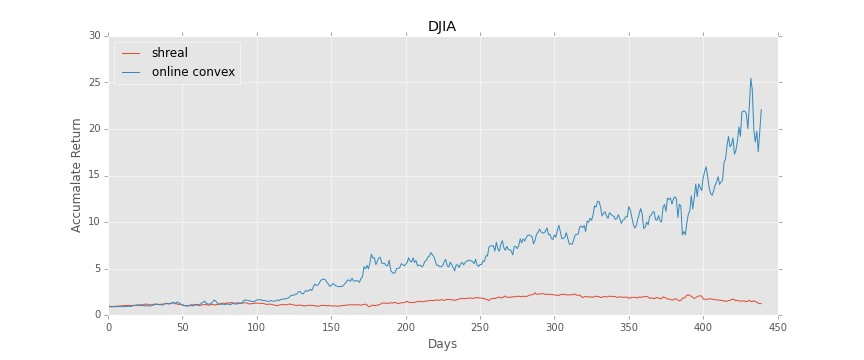
\includegraphics[width=1.0\columnwidth]{DJIA} 
\caption{Cumulative Wealth for SHREAL and Mirror Descent Algorithm on the DJIA Dataset without Transaction Costs.}
\label{DJIA}
\end{figure}

\begin{figure}[!h]
\centering
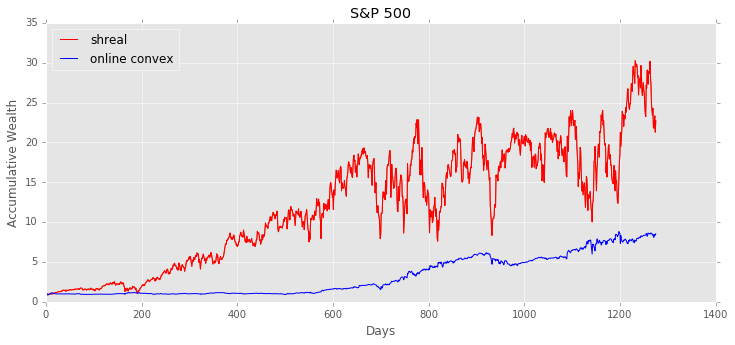
\includegraphics[width=0.85\columnwidth]{S_P500} 
\caption{Cumulative Wealth for SHREAL and Mirror Descent Algorithm on the S\&P 500 Dataset without Transaction Costs.}
\label{S_P500}
\end{figure}

\noindent Figure \ref{DJIA} and Figure \ref{S_P500} illustrate the performances of SHREAL and our Mirror Descent Algorithm on the above mentioned two datasets. The red line represents the results for the benchmark algorithm SHREAL and the blue line corresponds to that of our algorithm. It is clear that our algorithm outperforms SHREAL significantly under the poor market setting, where the accumulative wealth climbed steadily to more than 20 at the end of the 2-year period. The advantage of our algorithm in a good market scenario, where only a few stocks lost value, is less obvious. As shown in Figure \ref{S_P500}, although SHREAL achieved a higher return, its large and frequent fluctuations indicate higher risk compared with the stable growing pattern demonstrated by the Mirror Descent Algorithm. Results from both datasets show that our Mirror Descent Algorithm does a better risk control while giving desired return. 

\subsection{Manipulation of Parameters}

\begin{figure}[!h]
\centering
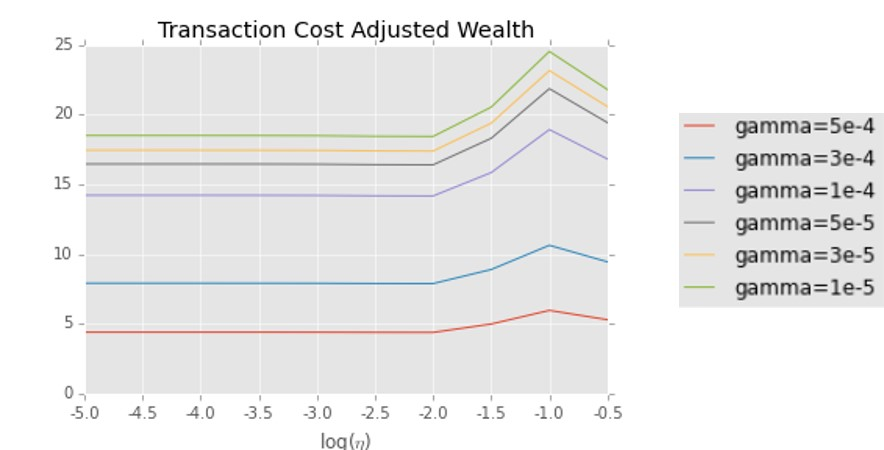
\includegraphics[width=0.85\columnwidth]{para} 
\caption{Cumulative Wealth for Mirror Descent Algorithm on the DJIA with Different transaction costs.}
\label{S_P500}
\end{figure}

\section{Conclusion}
In this project, we propose a Mirror Descent algorithm for online portfolio selection which takes into consideration of both leveraging and hedging. Moreover, we have added regularization terms for mean reversion theory and price momentum which better fit the market. Our experimental results shows that this Mirror Descent Algorithm provides strategies which can effectively control exposure to risk and lead to competitive return. It especially outperforms the SHREAL algorithm, which has been proven better than many state-of-the-art portfolio selection algorithms, in poor market.

\bibliographystyle{IEEEtran}
\bibliography{references_227}
\end{document}